\chapter{Objetivos} 
%----------------------------------------------------------------------------------------  que sirva como modelo a los alumnos de
%	SECTION 1
%--------------------------------------------------------------------------------------
El objetivo principal del TFG se centra en un entorno docente, ya que se han desarrollado un conjunto de practicas basadas en tecnologías web para la asignatura de LTAW. Para cada una de las practicas se ha preparado un enunciado tentativo y una solución de referencia convirtiéndose en subobjetivos que se describen en la siguiente lista.
\begin{enumerate}
\item  Crear un juego en la web basado en tecnologías del cliente. Para la visualización se utilizara Canvas mientras que para la funcionalidad se utilizara JavaScript permitiendo ejecutar eventos del teclado, además de incluir audio.
\item Crear un juego multijugador basado en tecnologías de comunicación bidireccional en tiempo real. Su diseño se basara en un servidor creado en NodeJS y WebSokects como mecanismo de comunicación bidireccional entre los navegadores y el servidor.
\item Crear un sitio Web de una tienda basada en tecnologías de servidor con manejo de base de datos. Su diseño se basara en el framework Django para la gestión del sitio de Web y como BBDD MySQL.
\item Crear una aplicación de Videoconferencia Peer-to-Peer entre navegadores basada en tecnologías de comunicación audiovisual. Su diseño se realizara con WebRTC como tecnología core y NodeJS para la creación del servidor auxiliar necesario.
\end{enumerate}
%----------------------------------------------------------------------------------------
%	SECTION 2
%----------------------------------------------------------------------------------------
\section{Metodología}
En La realización del proyecto se ha necesitado definir una metodología que permita planificar las tareas necesarias para llegar a nuestro objetivo. Por ello se ha seleccionado el modelo de desarrollo en cascada, figura \ref{fig:espiral}.

Este modelo define un conjunto de etapas distribuidas en cascada donde cada etapa tiene que terminarse por completo para pasar a la siguiente. A continuación, se explica en detalle cada etapa.
\begin{enumerate}
\item \textbf{Análisis de requisitos:} En esta fase se analizan las necesidades para determinar qué objetivos debe cubrir.
\item \textbf{Diseño del Sistema:} Descompone y organiza el sistema en elementos que puedan elaborarse por separado. Como resultado se obtiene la descripción de la estructura global del sistema y su especificación.
\item \textbf{Diseño del Programa:} Es la fase en donde se realizan los algoritmos necesarios para cubrir los requerimientos y analizar las herramientas necesarias para la etapa de Codificación.
\item \textbf{Codificación:} Es la fase en donde se implementa el código fuente, haciendo uso de prototipos así como de pruebas y ensayos para corregir errores.
\item \textbf{Pruebas:} Los elementos, ya programados, se ensamblan para componer el sistema y se comprueba que funciona correctamente y que cumple con los requisitos.
\end{enumerate}
Este esquema se aplica como ciclo de vida para desarrollar cada una de las practicas de las que trata el TFG.
\begin{figure}[!h]
\centering
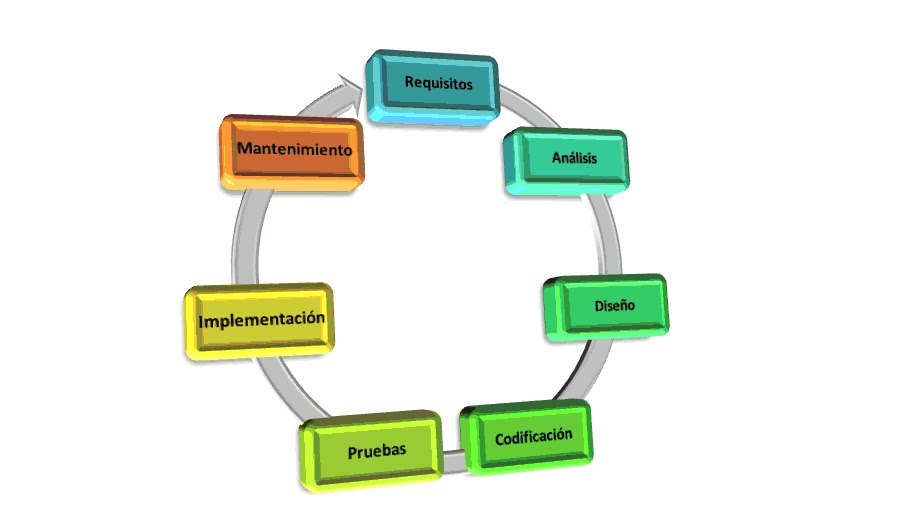
\includegraphics[width=0.8\linewidth]{Figures/cascada}
\decoRule
\caption[Metodología en cascada]{Metodología en cascada.}
\label{fig:espiral}
\end{figure}

Durante el tiempo que ha durado el proyecto se acordaron reuniones semanales con el tutor de forma presenciales o por Video-Conferencia en las que se revisaba los objetivos semanas y se definían los nuevos objetivos.

Los avances del proyecto se añadían a la \textbf{Mediawiki \cite{Mediawiki}} de JdeRobot. El contenido se divide en una sección de aprendizaje previo de tecnologías web con  pequeños ejemplos, la siguiente sección las características mas relevantes de las practicas así como un vídeo del resultado final de y finalmente una sección de vídeos mostrando la utilización de las aplicaciones por terceras personas. El código empleado en los ejemplos y practicas se encuentra en el repositorio de \textbf{GitHub \cite{Repositorio}}.
\section{Plan de trabajo}
Para llevar a cabo con éxito el desarrollo de las distintas practicas se definió el siguiente plan de trabajo.
\begin{enumerate}
\item \textbf{Fase de aprendizaje:} Esta primera etapa cubre el aprendizaje de diferentes tecnologías Web novedosas. Se dividió en tecnologías de cliente como JavaScript y HTML5, tecnologías de comunicación cliente-servidor como Ajax, formularios y WebSockets, tecnologías del servidor como NodeJS y  Django , BBDD como  MySql y MongoDB y por ultimo tecnologías de comunicación audiovisual como WebRTC.
\item \textbf{Diseño del enunciado de las practicas:} Con los conocimientos adquiridos de las diferentes tecnologías se realizo una propuesta del enunciado de cada practica. En cada enunciado recoge las tecnologías y requisitos que se tienen que cubrir durante el desarrollo.
\item \textbf{Implementación del enunciado de las practicas:} Tras validar el enunciado de cada practica se pasa al desarrollo siguiendo las pautas marcadas. Primero se diseña la solución que cubra los requisitos marcados para luego pasar a su implementación teniendo una visión general de los módulos, funciones y otros recursos que necesitan ser programados.
\item \textbf{Pruebas:} Cada una de las practicas han sido ejecutadas en distintos navegadores para evaluar su funcionalidad.
\end{enumerate}
